\begin{refsection}
\renewcommand{\thefigure}{\arabic{figure}}

\chapterTwoLines
{O patrimônio da Companhia de Jesus na capitania do Rio Grande do Norte}
{bens como sustento da fé (1600--1759)}
\label{chap:patrimonio}

\articleAuthor
{Ana Lunara da Silva Morais}
{Doutora pelo Programa Interuniversitário de Doutoramento em História (PIUDHist), vinculado ao Centro Interdisciplinar de História, Culturas e Sociedades (CIDEUHS), Universidade de Évora, Portugal. ID Lattes: 6721.3449.9390.7020. ORCID: 0000-0001-5401-3235. E-mail: lunara\textunderscore{}{}ana@hotmail.com.}

\begin{galoResumo}
    \marginpar{
        \begin{flushleft}
        \tiny \sffamily
        Como referenciar?\\\fullcite{SelfMorais2021}\mybibexclude{SelfMorais2021}, p. \pageref{chap:patrimonio}--\pageref{chap:patrimonioend}, \journalPubDate{}
        \end{flushleft}
    }
    A ordem religiosa Companhia de Jesus estabeleceu-se na capitania do Rio
    Grande desde o primórdio de sua colonização, no início do Seiscentos, onde atuou até a data de sua expulsão, em 1759. Nessa capitania angariaram muitas sesmarias, terras, pessoas escravizadas e cabeças de gado. Neste artigo, questiona-se de que forma os jesuítas angariaram e geriram seus bens no Rio Grande do Norte ao longo de mais de uma centúria e meia de atuação na capitania. Este trabalho é fruto de uma pesquisa de mestrado, para a qual se realizou o cruzamento de fontes de variados fundos, como o Arquivo Nacional da Torre do Tombo (ANTT), o Arquivo Histórico Ultramarino (AHU), o Arquivo Público Estadual de Pernambuco Jordão Emerenciano (APEPE) entre outros.
\end{galoResumo}

\galoPalavrasChave{Jesuítas. América portuguesa. Propriedade.}

\begin{otherlanguage}{english}

\fakeChapterTwoLines
{The patrimony of the Company of Jesus in the captaincy of Rio Grande do Norte} {property as a support of faith (1600--1759)}

\begin{galoResumo}[Abstract]
    The religious order Company of Jesus was established in the captaincy of Rio Grande since the principle of its colonization in the beginning of the Sixties, where it operated until the date of its expulsion, in 1759. In the captaincy of Rio Grande, they accumulate patrimony, sesmarias, lands, enslaved people and cattle heads. In this article, it is questioned how the Jesuits raised and managed their assets in Rio Grande do Norte over more than a century and a half of acting in the captaincy. This research, the result of a master's dissertation, that utilized sources from varied archives, especially the National Archives of Torre do Tombo (ANTT), the Overseas Historical Archives (AHU), the Public Archive of the Pernambuco State Jordão Emerenciano (APEPE) among others.
\end{galoResumo}

\galoPalavrasChave[Keywords]{Jesuits. Portuguese America. Property.}
\end{otherlanguage}

% \flourish

\section{Introdução}
A Companhia de Jesus começou a atuar no Brasil em 1549, quando juntamente com o governador geral do Brasil, Tomé de Sousa, desembarcaram alguns jesuítas. Os jesuítas tiveram uma importância fundamental desde o início da formação do império português devido a necessidade de oferecer suporte espiritual à colonização. Na América portuguesa, atuaram na conversão indígena, bem como no reforço da doutrina cristã junto aos colonos, atividades fundamentais para a consolidação de uma sociedade colonial em formação, colaborando para a fixação do povoamento.  

Os inacianos, para melhor se estabelecerem na colônia, passaram a angariar, por meio da compra e de doação régia ou particular, terras, pessoas escravizadas, entre outros bens. A ordem possuía uma visão pragmática da expansão comercial, percebendo-a como possibilidade de expansão da fé cristã, conseguindo para tal fim a obtenção de privilégios régios que colaboraram para o crescimento da ordem. A presença jesuítica na capitania do Rio Grande também ocorreu dessa forma. Ao longo do início do Seiscentos até a sua expulsão de todo o território português, em 1759, estabeleceram relevante patrimônio sob a justificativa de propagação da fé. A seguir será analisado de que forma a Companhia de Jesus angariou e geriu seus bens na capitania do Rio Grande do Norte ao longo de uma centúria e meia de atuação.  





\section{O patrimônio da companhia de jesus na capitania do Rio Grande do Norte}

Até o final do século XVI, a capitania do Rio Grande encontrava-se abandonada pela Coroa portuguesa, desprovida de qualquer assistência da mesma, e sujeita à ação de exploradores estrangeiros, pois as expedições colonizadoras haviam fracassado
\cites[][p.~200]{Medeiros1985}{Pereira2018}.

Em um contexto de efetivar a posse da colônia, já no final de 1597, organizou-se uma expedição à capitania do Rio Grande comandada pelo capitão-mor de Pernambuco Mascarenhas Homem, composta pelo capitão-mor da Paraíba Feliciano Coelho, o comandante de esquadra Francisco de Barros Rego, os irmãos mestiços Jerônimo, Antônio e Jorge Albuquerque, o franciscano Frei Bernardino das Neves, e os jesuítas padre Francisco Lemos e padre Gaspar de Samperes. A participação dos inacianos evidencia a sua importância no processo de consolidação da presença portuguesa na colônia \cite[p.~34]{MarizAndSuassuna2002}. 

Em janeiro de 1598, iniciou-se a construção do forte dos Reis Magos na barra do rio Potengi, sendo a planta elaborada pelo padre jesuíta Gaspar de Samperes. Fundou-se a cidade do Natal em 1599, e em 1600 procedeu-se o início das doações de sesmarias para efetivar o assentamento de colonizadores \cite[p.~24,~44]{Cascudo1984}. Segundo o padre provincial Pero Rodrigues, em 1599, os padres Gaspar de Samperes e Francisco Lemos fizeram entradas pelo rio Potengi para converter os índios e formar alianças com os Principais das aldeias. Estes padres erigiram cruzes onde os índios queriam reunir novamente seus membros, pois estavam dispersos devido aos conflitos com os portugueses, a chamada Guerra da Conquista \cite[Tombo~V,~p.~361--363]{Leite2004}. 

A distribuição de sesmarias --- título de doação de terra --- na capitania do Rio Grande iniciou-se em 1600, sendo concedidas pelo capitão-mor João Rodrigues Colaço. As informações sobre as doações de sesmaria no Rio Grande desde seu início até 1614, podem ser analisadas por meio do Translado do Auto de Repartição de Terras do Rio Grande \cite{Translado1909}. O rei Felipe II havia sido informado que, na capitania do Rio Grande, muitas terras haviam sido distribuídas para que fossem cultivadas e beneficiadas. Os sesmeiros não cumpridores das obrigações estipuladas, entretanto, geravam grandes perdas à Fazenda Real. Devido a este fato, o rei lançou um alvará em 8 de setembro de 1612, no qual requeria um levantamento sobre todas as terras que haviam sido doadas na capitania. As terras que se encontrassem abandonadas deveriam ser consideradas devolutas e riscadas dos livros de concessões, podendo ser doadas a outras pessoas \cite[p.~7--12]{Translado1909}. Além do descumprimento das obrigações, o rei reclamou principalmente sobre as imensas áreas doadas à Companhia de Jesus e aos filhos do capitão-mor do Rio Grande, Jerônimo de Albuquerque. O rei alegou que as terras não estavam sendo bem utilizadas e deveriam ser repartidas para outros sesmeiros \cite[p.~6--9]{Translado1909}.  

Das 186 datas de sesmaria doadas entre 1600 e 1614, cinco pertenciam à Companhia de Jesus, como se pode ver na figura \ref{fig:fig01} em sequência. As três primeiras datas concedidas foram doadas em 1600, pelo capitão-mor João Rodrigues Colaço, e são correspondentes às datas segunda, quarta e 24° do livro original de concessões. A primeira data localizava-se entre as ribeiras Arapapuhu e Itaorassutuba, com légua e meia de comprimento e uma de largura. No ato de realização de averiguação das terras, a Companhia cultivava nesta área roçarias e mantimentos, mas já havia criado gado vacum no local. A segunda data tratava-se de “uns chãos” de terra na cidade do Natal. A terceira data tratava-se de um sítio de salinas cercado que iniciava no estreito do rio Jaguarari (ou Iaguaribe) em direção ao sudoeste até chegar ao rio Aguape, também chamado de Obure, o qual se encontrava cercado pela ribeira do Potengi, com meia légua em quadra \cite[p.~19,~20~e~25]{Translado1909}.


\begin{figure}[ht]%
    \centering%
    \caption{Sesmarias da Companhia de Jesus na capitania do Rio Grande, início do século XVII}%
    \hspace*{-.025\textwidth}
    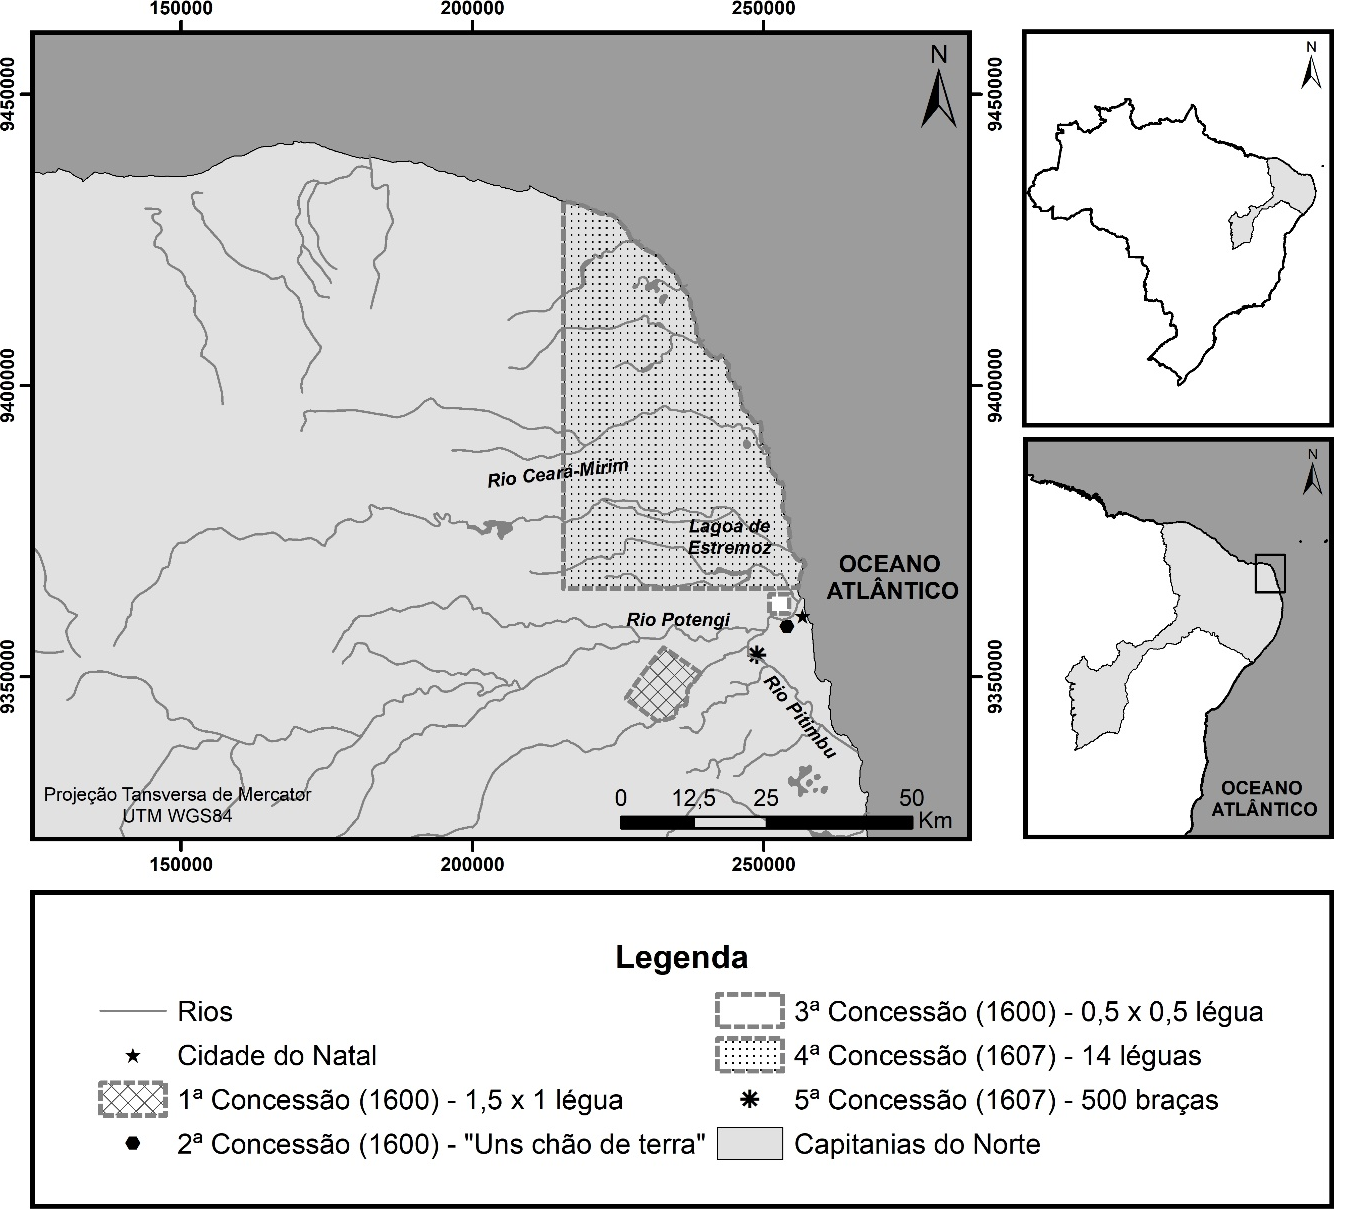
\includegraphics[width=1.05\textwidth]{articles/01-o-patrimonio-da-comp/fig01.png}%
    \caption*{Fonte: Elaboração própria a partir das informações contidas em: TRANSLADO, 1909.}%
    \label{fig:fig01}%
\end{figure}%

As outras duas datas de sesmarias foram concedidas pelo capitão-mor da capitania do Rio Grande, Jerônimo de Albuquerque, em 1607, e correspondem às datas número 102º e 103º do livro original de concessões. A primeira data localizava-se no “lugar chamado tijuru” (Guajiru), até o mar, podendo “compreender esta data quatorze léguas pouco mais ou menos”. Não há informações suficientes sobre os limites dessa sesmaria para realizar a sua delimitação, portanto, a área dessa concessão apontada na figura \ref{fig:fig01} é uma aproximação com base na extensão da mesma. Nessa sesmaria, a Companhia possuía dois currais de gado e quatro pessoas escravizadas originais da Guiné. A segunda data trata-se do aumento da primeira data de terra requerida pelos padres em 1600. Requereu-se os “sobejos que houvessem [de terras] que se achasse entre a data de Domingos Álvares e as dos padres”, sendo esta quinhentos braças --- equivalente a 1.100 metros, ou 0,16 légua em quadra --- de terras até chegar ao rio Pitimbu \cite[p.~49--51]{Translado1909}. 

Para Fátima Martins Lopes \citeyear[p.~107]{Lopes2003}, estas posses seriam a garantia do sustento dos padres da Companhia na capitania durante as missões volantes. O requerimento de um terreno na cidade do Natal fazia-se pela necessidade de os padres jesuítas formarem uma residência central, pois não havia muitos padres disponíveis, sendo impossível haver a quantidade necessária de padres para cada aldeia que deveria ser visitada. 

Ao requerer cinco datas de sesmaria, no entanto, tendo uma delas a grande extensão de 14 léguas, a Companhia de Jesus já deveria pensar sobre o crescimento da ordem na capitania do Rio Grande. Como foi explanado, as missões volantes eram periódicas e realizadas anualmente por apenas dois padres da Companhia. Assim, o requerimento de várias terras não representaria apenas a necessidade de garantir os mantimentos necessários para a subsistência dos padres na capitania. O exemplo das concessões de terra na capitania do Rio Grande aos inacianos corrobora as observações feitas pelos historiadores Edgard Leite \citeyear{Leite2000}, Paulo de Assunção \citeyear{Assuncao2004}, Maria Isabel da Silva Reis Vieira Rodrigues \citeyear{Rodrigues1997}, e Manoela Pedroza \citeyear{Pedroza2020} que atentaram para a ideia de que a Companhia de Jesus possuía a fé como justificativa para a ampliação de suas atuações. 

Cabe apontar que não se sabe o destino das terras concedidas aos jesuítas na capitania do Rio Grande na primeira década de 1600. O alvará de 1612 ordenou a diminuição da terra da Companhia do lugar chamado Tijuru, possivelmente Guajiru, nas proximidades da aldeia e lagoa de mesmo nome. Contudo, não se sabe o que aconteceu com as terras após a invasão holandesa e a fuga dos padres inacianos juntamente com outros moradores da capitania. Quando os inacianos retornaram à capitania do Rio Grande, depois de 1678, não há informações sobre a posse das terras doadas entre 1600 e 1607. Verificou-se, entretanto, que das cinco sesmarias doadas no início do século XVII encontrava-se nas posses da Companhia no momento de sua expulsão algumas fazendas de gado ainda localizadas na área de sesmarias de maior extensão.  

Fátima Martins Lopes \citeyear{Lopes2003} destacou que apesar das dificuldades enfrentadas pelos moradores na capitania, como a hostilidade dos índios e também pela natureza da região (falta de água, e solo arenoso), houve uma adequação às condições da capitania. Explorou-se o sal natural, foram criados gado e outros animais, desenvolveu-se pescarias e coletas de âmbar, e foram produzidos alimentos. A capitania do Rio Grande não possuía alfândega, assim não comercializava os seus produtos diretamente com Portugal, e sim por Pernambuco A capitania possuía apenas um engenho de cana-de-açúcar no período, o Cunhaú, não havendo uma produção de açúcar relevante. Além disso, é possível que pelo destaque na produção de alimentos, a capitania tenha comercializado internamente com as capitanias próximas, pois havia um livre comércio entre estas \cites[p.~191--196]{Dias2011}[p.~203--225]{Dias2018}. 

As terras requeridas pela Companhia podem ser associadas às atividades já referidas, pois se tratam de um sítio de salinas no litoral, ribeiras de rios importantes para currais de gado e cultivo de mantimentos. A presença de africanos escravizados em uma das concessões mostra o interesse dos jesuítas em iniciar uma atividade produtiva ou mesmo preparar e melhorar suas terras.  

Ao analisar o Translado do Auto de Repartição de Terras do Rio Grande, Lopes \citeyear[p.~103]{Lopes2003} observou que das 186 datas, apenas em sete havia referência sobre a presença de pessoas escravizadas nas terras, das quais apenas em duas fazia-se menção à posse de pessoas escravizadas da Guiné, sendo uma delas a da Companhia de Jesus. Segundo Lopes \citeyear[p.~68]{Lopes2003}, a escravidão negra no século XVII foi uma realidade para a Bahia e Pernambuco, capitanias açucareiras que podiam importar pessoas escravizadas, diferentemente do Rio Grande, onde a opção pela escravidão negra era muito restrita. Pesquisas mais recentes evidenciaram a presença da escravidão negra na capitania do Rio Grande somente para o final do século XVIII e início do século XIX \cites{Macedo2007,Souza2013}. Neste aspecto, a posse de pessoas escravizadas pela Companhia mostra que a ordem era privilegiada se comparada à situação dos demais moradores.  

Com a volta dos jesuítas à capitania após a expulsão dos holandeses, retomou-se o objetivo de catequizar os índios da região. Segundo Serafim Leite, “quebrando-se o julgo holandês, restabeleceu-se as atividades jesuíticas no Rio Grande, quer como feição econômica e rural, quer como a vida catequética nos aldeamentos de Guajiru e Guaraíras” \cite[Tombo~V,~p.~370]{Leite2004}. Dessa forma, além das atividades missionárias nos aldeamentos --- refere-se a um aglomerado resultante da “aculturação” mediante a presença de missionários catequistas \cite[p.~39]{Azevedo1957} --- os jesuítas também atuaram nas atividades econômicas da capitania.

Posteriormente à expulsão dos holandeses, as missões volantes ocorreram anualmente com a visita de dois padres do Colégio de Olinda da Companhia de Jesus. Atuaram formando alianças com os índios e batizando-os. Durante os contatos iniciais na capitania do Rio Grande, a habilidade intercultural dos jesuítas e o papel de intermediários, possibilitaram as alianças com os Potiguara. Os jesuítas tornaram-se mais eficientes que as forças militares, pois, possuíam melhores estratégias da aproximação, tendo possibilitado o encontro pacífico com os índios \cite[p.~88]{Porto2000}. 

Não há muitas informações acerca da atuação jesuítica na capitania do Rio Grande no período da ocupação holandesa (1633--1654). É sabido que até 1634, entretanto, os missionários visitaram algumas aldeias, mas após esta data, não há registro dos inacianos atuando na capitania \cite[p.~91]{Porto2000}. Com a expulsão dos holandeses, retomou-se o processo de colonização portuguesa na capitania: o Senado da Câmara de Natal foi restabelecido; as sesmarias passaram a ser doadas novamente; e posteriormente os jesuítas retornaram à capitania.  

Desde o Plano Civilizador do padre provincial Manuel da Nóbrega no governo de Mem de Sá, iniciou-se uma mudança na forma de catequizar os índios. Os jesuítas perceberam que a missão volante havia se tornado menos eficaz mediante a necessidade de melhor concentrar os índios e pregar a doutrina cristã, fazendo os índios abandonarem os seus hábitos culturais e tornarem-se cristãos. As missões efetivas, chamadas apenas de missões, aldeavam os índios buscando aproximar-se do ambiente natural dos mesmos, e simultaneamente visavam o seu afastamento dos centros de colonização \cite{Azevedo1959}. Tais missões também deveriam possuir uma organização administrativa, deveriam inserir os índios no trabalho agrícola, promover a ida à igreja, entre outras obrigações \cite[p.~162]{Lopes2003}. 

Este novo modo de catequizar os índios foi ao encontro dos interesses das autoridades da capitania, pois com a expulsão dos holandeses, a retomada da colonização na região expandiu-se para o interior, seguindo as frentes de penetração pecuária que provinham da Paraíba, Pernambuco e Ceará \cite[p.~129]{Lopes2003}. Ao direcionarem-se para o sertão --- aqui é compreendido como espaço sem atuação da Coroa portuguesa \cite[p.~112]{Silva2010} --- os colonos depararam-se com vários grupos indígenas, os quais foram resistentes à colonização portuguesa, gerando a Guerra dos Bárbaros \cites[p.~96]{Cascudo1984}{Dias2015}{Silva2015}.  

Neste contexto de conflitos entre índios e colonos e a necessidade de estender as posses de terras para a criação de gado, coube aos jesuítas aldear os índios para que estes fossem reduzidos em missões e fossem “apaziguados”. Nestas missões também se tentou regularizar a mão de obra indígena \cite[p.~95]{Porto2000}. 

Os jesuítas fixaram duas missões efetivas na capitania do Rio Grande. Ambos aldeamentos eram de remanescentes Potiguara, entre outras etnias: São Miguel de Guajiru e São João Batista das Guaraíras. O aldeamento de Guajiru estava localizado na margem da lagoa de mesmo nome (atual lagoa de Extremoz), a duas léguas da cidade do Natal, e foi relatada sua existência desde 1641, por um emissário holandês. Tal aldeamento, portanto, localizava-se na sesmaria de enorme extensão de 14 léguas concedida no início do século XVII a Companhia de Jesus. A presença dos jesuítas na aldeia foi mencionada a partir de 1679, por meio de uma queixa dos oficiais da Câmara da cidade do Natal ao bispo de Pernambuco, na qual acusavam o padre inaciano João de Gouveia de incitar os índios contra um administrador colonial. Entretanto, o primeiro relato oficial sobre a presença dos jesuítas na aldeia foi apenas em 1683, no Catálogo da Companhia de Jesus, sendo o seu superior o padre Antônio Cardoso, na qual também estava presente o padre Francisco de Albuquerque \cite[p.~170]{Lopes2003}.  

A presença jesuítica no aldeamento de Guaraíras, localizado nas proximidades do rio Jacu, foi relatada desde 1681, pois neste ano ordenou-se que os índios da aldeia de Mipibu fossem reunidos com os índios do aldeamento de Guaraíras \cite[p.~35]{Lemos1912}. A missão foi registrada nos Catálogos da Companhia de Jesus em 1683, com a presença do padre superior Luiz Pinto e do padre José dos Reis \cite[p.~172]{Lopes2003}.  

Foram nos aldeamentos de Guajiru e Guaraíras, e em suas proximidades, que a Companhia de Jesus exerceu as suas atividades de forma mais intensa. Ao fundar uma missão fixa, os jesuítas deveriam preocupar-se com o sustento da ordem, bem como de seus membros e dos índios. Houve a necessidade da fundação de fazendas para a produção de mantimentos, e criação de animais. A forma como os jesuítas administravam as atividades produtivas nos aldeamentos e em suas fazendas, pode ser percebida por meio da análise de suas posses de terra e dos conflitos derivados desta prática.  

Com o Alvará de 23 de novembro de 1700, que garantiu uma légua de terra em quadra (uma légua -- 6,6 km -- de comprimento por uma de largura) para o sustento dos índios e missionários, as missões Guajiru e Guaraíras tiveram suas terras demarcadas na primeira década do século XVIII \cites[p.~111--112]{Cascudo1984}[p.~44]{Lopes2005}.  

Além das terras das missões, que pertenciam aos índios nelas aldeados, mas que também eram usufruídas pelos inacianos, observou-se por meio de algumas cartas de sesmarias que apontavam os jesuítas como confrontantes de suas terras, que a Companhia de Jesus possuía outras terras na capitania do Rio Grande.   

Antônio Cardoso Batalha solicitou uma terra nas proximidades da ribeira do Ceará-Mirim, em 1739, e afirmou que a terra chamada Maracacheta, localizada nas proximidades do rio Ceará-Mirim, em direção à praia (litoral leste da capitania) pertencia aos Jesuítas.\footnote{Instituto Histórico e Geográfico do Rio Grande do Norte [IHGRN] --- Fundo Sesmarias, Livro IV, n. 287, fl. 51--52.} Acredita-se na possibilidade de o lugar Maracacheta ter alguma relação com o lugar chamado Massangana, localizado ao norte da missão de Guajiru.  

O padre jesuíta Antônio de Amorim, em agosto de 1736, requereu um novo documento da sesmaria que herdou de seu pai, o coronel Antônio Dias Pereira. A petição foi feita por intermédio do procurador do suplicante, o padre jesuíta coadjutor e licenciado João Gomes Freire. A terra requerida localizava-se nas confrontações das terras da própria Companhia de Jesus, nas proximidades do rio Ceará-Mirim, seguindo o curso do rio Caratã --- hoje rio Mudo, ou rio do Jorge, o qual deságua na lagoa de Extremoz, antiga lagoa de Guajiru \cite[p.~79]{Cascudo1968} --- ficando este no meio das terras de um lugar chamado Cacimbas.\footnote{IHGRN --- Fundo Sesmarias, Livro III, n. 241, fl. 158--159.} Esta sesmaria pode revelar não apenas uma terra da Companhia nas proximidades da missão de Guajiru, como também pode evidenciar a anexação da terra herdada por um membro da Companhia, visto que quem realizou a petição foi outro padre jesuíta e a terra localizava-se nas confrontações de outras terras da ordem. Ao catequizar os índios nas ditas missões, os jesuítas utilizaram-se das terras das mesmas, bem como das terras que haviam requerido inicialmente para as fazendas que produziam mantimentos e tinham criações de gado para efetivar a catequização.  

Para a identificação das posses jesuíticas na capitania do Rio Grande na primeira metade do século XVIII realizou-se a análise de fontes referentes ao estabelecimento do Diretório dos Índios. Esse, decretado em 8 de maio de 1758, aboliu o poder temporal e espiritual dos missionários sobre os índios aldeados. Desta forma, os inacianos deveriam ser substituídos pela administração civil e pelo clero secular \cite[p.~18--20]{Couto1990}. Em 14 de setembro do mesmo ano, Luís Diogo Lobo da Silva, governador das Capitanias do Norte, ordenou que fossem erigidas vilas nos aldeamentos administrados pelos jesuítas \cite[p.~43--46]{Couto1990}. No início do ano de 1759, Dom Francisco Xavier Aranha, bispo de Pernambuco, ordenou aos superiores dos Colégios de Olinda e Recife, que quando os substitutos seculares chegassem às missões os jesuítas deveriam se retirar das mesmas e se dirigissem aos seus Colégios \cite[p.~102]{Lopes2005}. 

Em junho de 1759, os párocos seculares chegaram às missões do Rio Grande, e realizou-se um alistamento dos bens pertencentes às missões, às igrejas e às residências jesuíticas. Os bens móveis dos jesuítas passaram a ser subordinados à jurisdição do arcebispo de Olinda, visto que seu caráter religioso impedia que a Coroa os confiscasse. Assim, o rei permitiu que tais bens ficassem sob a responsabilidade do arcebispo de Olinda, o qual deveria sequestrar e repartir tais bens \cite[p.~29--35]{Couto1990}. O ouvidor geral Bernardo Coelho da Gama e Casco ordenou que se realizasse o inventário dos bens das missões jesuíticas da capitania do Rio Grande, Guajiru e Guaraíras, em 1760, os quais foram registrados em 1761 \cite[p.~172]{Lopes2005}. 

O padre inaciano Alexandre Carvalho entregou os bens da igreja da antiga missão de Guajiru, Nossa Senhora dos Prazeres e São Miguel, para o vigário Antônio de Souza Magalhães. No inventário, que se encontra no códice 1964 do Arquivo Histórico Ultramarino (AHU), os bens da igreja eram compostos por 17 imagens religiosas, das quais sete apresentavam adornos de prata, e uma de ouro; vários objetos destinados para a celebração de missas, dos quais alguns eram de prata como relicários, vasos de comunhão, cálices e turíbulo; toalhas, cortinas, mantos, capas, véus, missais, entre outros. A construção da igreja de Nossa Senhora dos Prazeres e São Miguel ainda não estava concluída no momento do inventário.\footnote{Arquivo Histórico Ultramarino [AHU] --- Códice 1964, fl. 337--342. Inventário que mandou fazer o Dr. Desembargador ouvidor geral Bernardo Coelho da Gama e Casco, de Todos os Bens Pertencentes a esta missão de Guajiru e igreja de Nossa Senhora dos Prazeres e São Miguel.} 

A missão de Guajiru possuía 70 cabeças de gado vacum e nove de cavalar. Também possuía 15 pessoas escravizadas.\footnote{AHU --- Códice 1964, fl. 337--342.} Como os missionários não possuíam comprovantes da origem da posse pessoas escravizadas, nem de seus gados, o ouvidor geral da Gama e Casco instaurou um sumário de testemunhas para que fosse apurado se estas propriedades pertenciam à missão ou à Companhia de Jesus. Segundo alguns índios, antigos moradores da missão, as pessoas escravizadas eram descendentes dos cativos que os missionários haviam comprado ou trazido nos primórdios da missão.\footnote{AHU --- Códice 1964, fl. 343--347. Auto de Sumário que mandou fazer Bernardo Coelho da Gama e Casco para por ele perguntar testemunhas ex-ofício, em 30/05/1760.} 

Na missão de Guaraíras, os bens foram passados ao vigário Pantaleão da Costa de Araújo pelo padre jesuíta Manoel Pinheiro. A igreja de São João Batista encontrava-se nova, construída de pedra e cal. Os bens pertencentes a esta igreja, embora possuíssem menos imagens religiosas com adornos de prata em comparação à missão de Guajiru, possuía mais bens. Havia pias de água benta, pia batismal, dois confessionários, e ainda uma grande variedade de utensílios religiosos e adornos decorativos: galhetas, cruzes, cálices de prata, castiçais, velas, bandeiras de paniconografia (gravura em relevo sobre zinco), e panos, mantos, cortinas e vestimentas sacerdotais de tecidos nobres. A missão ainda possuía 174 cabeças de gado vacum, 57 de cavalar, 27 de gado caprino, 38 de ovino, três porcos, e mais vinte e três mil e setecentos réis.\footnote{AHU --- Códice 1964, fl. 390--398. Inventário que mandou fazer o Dr. Desembargador ouvidor geral Bernardo Coelho da Gama e Casco, de todos os bens pertencentes a esta missão de guariras e igreja de São Sebastião.}  

A missão de Guaraíras possuía pertences que podem refletir uma melhor condição dessa missão em comparação à missão de Guajiru. A missão de Guaraíras possuía uma livraria com 20 volumes, e interessantes utensílios como “uma chocolateira e seu pau”, um “baú de Moscóvia”, e “umas charamelhas” (instrumento de sopro).\footnote{AHU --- Códice 1964, fl. 390--398.} 

Ambas as residências das missões possuíam uma mobília básica como cadeiras, mesas, tamboretes, e objetos de higiene pessoal. Em ambos os inventários também se percebe instrumentos de trabalho, relacionados à produção econômica desempenhada pelos índios, como redes de pescas, serrotes, entre outros \cite[p.~173]{Lopes2005}. 

Assim, como havia sido acordado anteriormente, desde maio de 1758, os bens semoventes (ornamentos, utensílios, animais, pessoas escravizadas, entre outros) das missões jesuíticas foram divididos em 1761, conforme a proposta lançada pelo bispo de Olinda à junta criadora das vilas, que incluía representantes eclesiásticos, funcionários coloniais e índios que ocupavam cargos civis e militares \cite[p.~179]{Lopes2005}. Os bens de raiz das missões, ou seja, as terras que foram concedidas para a criação da missão ou mesmo para a ampliação de sua extensão, deveriam ser repartidas entre os índios das mesmas de acordo com o arcebispado, e o governador ou capitão-mor da capitania, não ficando nenhuma terra para a igreja.\footnote{Arquivo Público do Estado de Pernambuco [APEPE] --- Ordens Régias, Livro nº 10 (1755--1760), fl. 144--146. }

As providências para erigir as novas vilas começaram no início do ano de 1759. As missões de Guajiru e de Guaraíras tornaram-se respectivamente as vilas de Estremoz em 3 de maio de 1760, e a vila de Arêz em 15 de junho de 1760 \cite[p.~122--123]{Lopes2005}. Nesta mudança de missões para vilas, também foi ordenado que o ouvidor geral Bernardo Coelho da Gama e Casco convocasse os prelados dos Colégios de Olinda (ao qual estavam submetidas às missões jesuíticas do Rio Grande), Recife e Paraíba, para que fossem apresentados os bens que os jesuítas possuíam em um prazo de 20 dias após a averiguação e levantamento dos bens.\footnote{APEPE --- Ordens Régias, Livro nº 10 (1755--1760), fl. 144--146.} 

Desde maio de 1758, o rei havia ordenado que os bens de raiz pertencentes à Companhia de Jesus que estivessem em desacordo com as antigas leis impostas a ordens religiosas poderiam ser sequestrados. Assim, os bens de raiz que não possuíssem licença régia --- norma referente ao Título XVIII das Ordenações Filipinas, presente no alvará de 30 de julho de 1611, no qual se ordenou que todos os bens religiosos deveriam possuir sua respectiva autorização --- poderiam ser de imediato revertidos à Coroa portuguesa. Em agosto de 1759, o rei Dom José ordenou que fosse realizado o sequestro de todos os bens da Companhia de Jesus em Pernambuco com sua respectiva origem e valor.\footnote{Arquivo Nacional da Torre do Tombo [ANTT] --- Documentação das capitanias do Brasil existente no núcleo do Real Erário, Livro nº 574, documento sem número. }

Assim, averiguaram-se alguns bens de raiz da Companhia de Jesus na capitania do Rio Grande pertencentes então ao Colégio de Olinda. O ouvidor Gama e Casco arrolou alguns bens de raiz e os colocou em arrematação pública para serem arrematados em 1º de junho de 1760 --- a saber as fazendas: Oitizeiro, Ceará e Curral de Baixo.\footnote{AHU-PE --- Papéis Avulsos, Cx. 95. Doc. 7493. Ofício do ouvidor geral Bernardo Coelho da Gama e Casco ao secretário de Estado Conde de Oieiras. 10 de fevereiro de 1761.} É sabido que além dessas fazendas os inacianos possuíam na capitania do Rio Grande os sítios Galos e Guamaré e uma fazenda de gado chamada de Santa Cruz,\footnote{AHU-PE --- Papéis Avulsos, Cx. 95. Doc. 7493.} como se pode ver na figura \ref{fig:fig02}.  

Segundo José Jorge da Costa Couto, enquanto Portugal negociava com a Cúria de Roma (1759-1760) acerca da situação dos bens jesuíticos, a administração de Portugal manteve os bens fundiários da ordem jesuítica intocáveis, com exceção dos bens que não possuíam licença régia \cite[p.~149]{Couto1990}.   

Com a definitiva expulsão dos jesuítas de Portugal e de todos os seus domínios, em 3 de setembro de 1759, os bens da Companhia de Jesus foram revertidos à Coroa, visto que a ordem religiosa foi extinta. Tal fato foi corroborado pelo alvará de 25 de fevereiro de 1761, o qual determinou a imediata incorporação no fisco da Câmara Real de todos os bens temporais, isto é, aqueles que não se encontravam direta e exclusivamente destinados ao culto divino \cite[p.~151]{Couto1990}. 

Desse modo, a ordem régia de 22 de outubro de 1761 estabeleceu como os bens confiscados dos jesuítas deveriam ser classificados, registrados e arrematados. Os bens imóveis deveriam ser alienados em público, com a presença da Junta congregada, sendo aceito o maior lance dos sujeitos interessados em arrendar o bem. A arrematação poderia ser paga em dinheiro ou em gêneros de fácil venda \cite[p.~153]{Couto1990}. As normas da referida ordem chegaram ao governador de Pernambuco, e consequentemente para as Capitanias do Norte, apenas em 1763. 

\begin{figure}[ht]%
    \centering%
    \caption{As terras da Companhia de Jesus na data de sua expulsão (1759)}%
    \hspace*{-.025\textwidth}
    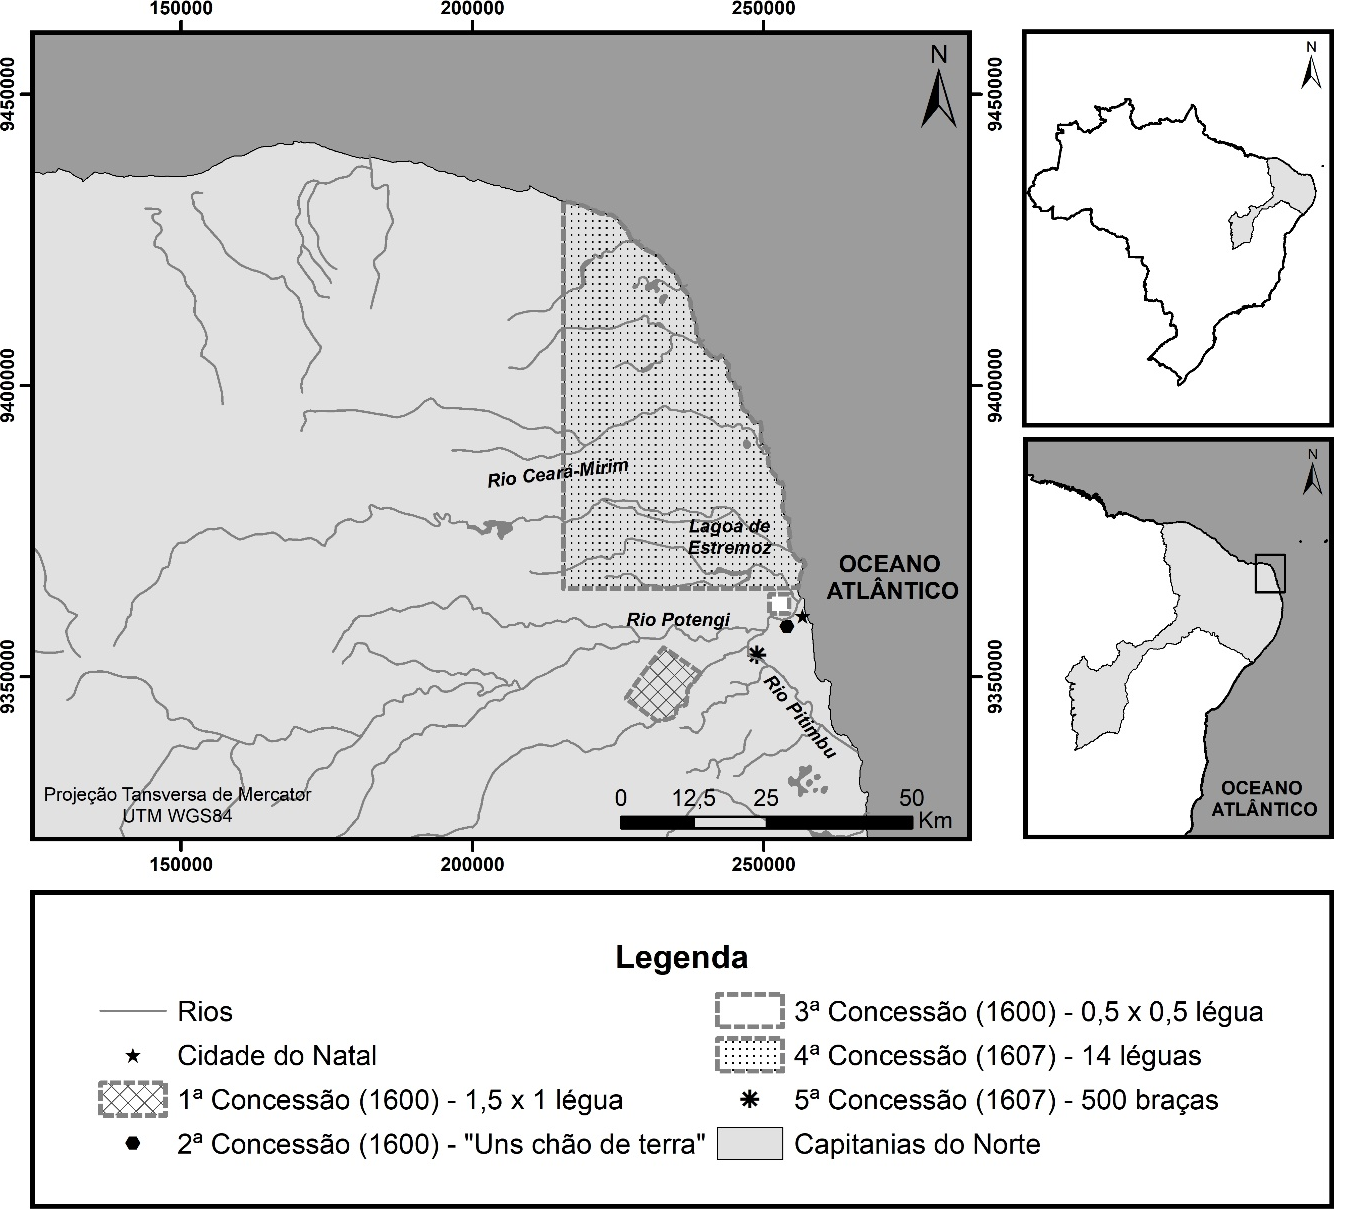
\includegraphics[width=1.05\textwidth]{articles/01-o-patrimonio-da-comp/fig01.png}%
    \caption*{Fonte: Elaboração própria a partir das informações contidas em: IHGB --- Arq. 1.1.15. Avaliações dos bens jesuítas em Pernambuco, 1772. AHU-PE --- Papéis Avulsos, Cx. 95. Doc. 7493. 10 de fevereiro de 1761. }%
    \label{fig:fig02}%
\end{figure}%

Foi criada, em 10 de abril de 1769, uma Junta da Fazenda Real em Pernambuco, para evitar falhas na administração e arrecadação da Real Fazenda de Pernambuco. A mesma era composta pelo governador, procurador, provedor e contador da Fazenda. A Junta deveria ser responsável por classificar os bens confiscados bem como elaborar um livro de inventário dos ditos bens \cite[p.~158]{Couto1990}. 

Foi por meio destes documentos produzidos pela Junta da Fazenda Real em Pernambuco que é sabido que, em 1772, algumas fazendas jesuíticas no Rio Grande, pertencentes ao Colégio de Olinda, não estavam arrematadas: fazenda Oitizeiro; fazenda Ceará; fazenda Curral de Baixo; sorte de terras no lugar chamado Ceará; e sítio de terra chamado Arraial das Formigas na ribeira do rio Piranhas.\footnote{Instituto Histórico e Geográfico Brasileiro [IHGB] --- Arq. 1.1.15. Avaliações dos bens jesuítas em Pernambuco, 1772, p. 9--11.} 

As fazendas Oitizeiro, Ceará, e Curral de Baixo, as quais haviam sido arrematadas a Antônio da Silva de Carvalho em 1760, ficaram deterioradas após o falecimento do mesmo. As ditas três fazendas passaram novamente para a administração da Provedoria da Fazenda do Rio Grande, em 1770, e foram leiloadas em 1776 para Domingos Gomes Maciel.\footnote{ANTT --- Erário Régio, Capitanias do Brasil --- Pernambuco, livro 636, traslado nº 3, Autos de arrematação dos bens confiscados dos jesuítas e pertencentes ao Fisco Real, dos anos de 1776, 1777 e 1778. Em carta da Junta de Pernambuco, de 15 de junho de 1779.}  

As posses de terras da Companhia de Jesus na capitania do Rio Grande as quais se tem conhecimento foram as fazendas Oitizeiro, Ceará, Curral de Baixo e Santa Cruz; os sítios dos Galos, Guamaré, e o Arraial das Formigas; além de uma sorte de terra no lugar chamado Ceará; totalizando três fazendas, dois sítios, um arraial e uma sorte de terra. Como os bens imóveis citados, referentes às missões de Guajiru e Guaraíras, estavam subordinados a mesma jurisdição do Colégio jesuítico de Olinda, não se conseguiu verificar por meio da documentação analisada quais fazendas estavam subordinadas à administração específica dos padres da missão de Guajiru, com exceção da fazenda Santa Cruz.\footnote{AHU --- Códice 1822, fl. 31v--32, CARTA do capitão-mor do Rio Grande, João Coutinho de Bragança ao governador de Pernambuco, em 17/02/1760.}

\section{Os bens como sustento da fé}

Segundo o historiador Fabricio Lyrio Santos \citeyear{Santos2008} as práticas inacianas de acumulação de bens não contradiziam o voto de pobreza dos membros da ordem. Essa concepção acerca da acumulação de bens para o desenvolvimento das atividades da ordem inaciana estava presente já na versão sumária das regras de funcionamento da ordem, aprovada pelo Papa Paulo III em 1540, na qual o fundador da Companhia de Jesus, padre Inácio de Loyola, recomendava o voto de pobreza, mas, permitia que se aceitassem rendas para o sustendo dos estudantes \cite{Santos2008}.  

Além disso, as cartas apostólicas \textit{Regimini militantis Ecclesiae}, de 27 de setembro de 1540, e \textit{Exposcit debitum}, de 21 de julho de 1550, corroboravam as regras de criação da ordem e aceitavam que a mesma estabelecesse colégios para formação de estudantes e novos membros da ordem. Tais colégios deveriam possuir suas próprias rendas e/ou propriedades para sua manutenção e sustento de seus membros \cite{Santos2008}. Portanto, poderiam ou deveriam ser aceitas as doações régias para efetivar o funcionamento da ordem jesuítica.  

Segundo Edgard Leite \citeyear[p.~60]{Leite2000}, a história da Companhia de Jesus no Brasil é a história da construção de um gigantesco patrimônio, o qual foi construído por uma série de privilégios e favorecimentos da Coroa portuguesa, e também por decisão acordada dentro da própria ordem. 

Desde o primeiro ano que os jesuítas chegaram ao Brasil, em 1549, receberam benefícios, bem como muitos colonos \cite[p.~30--71]{Fragoso2001}. No dito ano, a bula papal \textit{Licet Debitum} isentou o pagamento de dízimos \cite[Tombo~VII,~p.~103]{Leite2004}. Tal isenção foi confirmada no reinado de Dom Sebastião posteriormente em 1576 e 1577. Também foi estabelecido, desde o princípio das ações jesuíticas, o fornecimento de gêneros à Companhia, com finalidade de manter as necessidades da ordem. A partir de 1560 e 1570, uma porcentagem dos impostos arrecadados pagos em açúcar à Coroa, a redízima dos dízimos, era repassada aos três colégios jesuíticos do Brasil: Bahia, Rio de Janeiro e Olinda. Em 1573, um alvará isentou a Companhia dos pagamentos de direitos alfandegários sobre os produtos que recebessem na ou enviassem da América portuguesa. A Coroa também destinava aos jesuítas a subvenção pessoal, equivalente a uma pensão anual, para aqueles que embarcavam de Portugal para o Brasil, sendo 20.000 réis em 1581, e 35.000 réis em 1690 \cite[p.~60--61]{Leite2000}. 

Além dos subsídios reais, com a reconhecida necessidade da posse de terras para o sustento da ordem jesuítica, bem como para a formação de núcleos territoriais, os membros da Companhia obtiveram terras por meio das seguintes formas: sesmaria, doação, compra, e mais raramente a troca \cite[p.~12]{Alveal2002}. As doações de fiéis podiam ocorrer pela estipulação de um valor a ser doado à Companhia anualmente, em espécie ou em produtos do mercado colonial \cite[p.~81]{Assuncao2004}. 

Os subsídios reais e as isenções de pagamentos de dízimos e taxas alfandegárias mostraram o interesse da Coroa portuguesa de livrar a ordem de obrigações, proporcionando não apenas o seu mantimento, como também o seu crescimento. Para a Coroa, a presença jesuítica, naquele momento, era não apenas favorável como necessária, pois, convertia-se o gentio e controlava-se a mão de obra indígena, combatia-se a ação de invasores estrangeiros e relatava-se a presença destes, e, sobretudo, confirmava a presença portuguesa no novo território \cite[p.~156]{Assuncao2004}. Assim, esse importante papel da Companhia de Jesus na integração do mundo colonial era percebido como um serviço prestados à Coroa. 

Ao descrever sobre os bens da Companhia, o historiador e padre jesuíta Serafim Leite relatou que, à primeira vista, os bens da Companhia geram uma visão equivocada da ordem. Ele afirma que o equívoco é desfeito quando percebida a necessidade dos bens para a manutenção da Companhia. Segundo o autor, os jesuítas não obtinham lucros das atividades que exercitavam, apenas necessitavam de maiores subsídios para continuarem com as atividades missionárias \cite[Tombo~I,~p.~49]{Leite2004}.

Assim como Serafim Leite, Dauril Alden não corrobora a ideia de que a Companhia de Jesus se utilizou do comércio e de outras estratégias para manter a ordem religiosa. Ambos os autores afirmam que a Companhia não havia quebrado o voto de pobreza. Alden defende que a Companhia de Jesus não obteve ganhos significativos, e contesta a associação entre jesuítas e homens do comércio moderno, comumente realizada. Para Alden \citeyear[p.~527]{Alden1996}, as atividades desenvolvidas pela Companhia não se enquadravam como comércio.  

Entretanto, autores como Paulo de Assunção \citeyear{Assuncao2004}, Edgard Leite \citeyear{Leite2000}, Maria Isabel da Silva Reis Vieira Rodrigues \citeyear{Rodrigues1997} e Manoela Pedroza \citeyear{Pedroza2020}, demonstraram por meio de suas pesquisas que a Companhia de Jesus possuía a fé como justificativa para a ampliação de suas atuações, principalmente no comércio de gêneros alimentícios. Por meio do apoio da Coroa, de concessões de terras, das doações de fiéis, e da administração de seus bens, a Companhia construiu no Brasil um grande e poderoso patrimônio.   

Os jesuítas, inseridos em uma sociedade colonial em formação, acabaram por se adequar àquela sociedade. A mentalidade moderna do descobrimento e da conquista não influenciou apenas a monarquia e os colonos. Os jesuítas, ao compartilharem um mesmo espaço de relações sociais, incorporaram valores modernos em suas atuações, tornando-se necessário para o desenvolvimento da ordem, a inserção dos jesuítas no mundo mercantilista \cite[p.~239]{Assuncao2004}. Deste modo:

    \begin{quote}
    A preocupação com o cultivo e a exploração das terras de forma a garantir a estrutura da Companhia colocou-a em consonância com a lógica da colonização da época moderna. O empreendimento jesuítico era parte de uma ação colonizadora que almejava, por meio da circulação de mercadorias, efetivar o poder da fé. \cite[p.~251]{Assuncao2004}         
    \end{quote}

Os jesuítas designados a missionar na América portuguesa encontravam-se inseridos em um novo mundo que, diferentemente do contexto europeu, havia necessidades e dificuldades específicas reveladas pelo meio: a produção de alimentos, as pragas e pestes nos roçados, guerras entre etnias indígenas, invasões estrangeiras, entre outras. Mesmo com os subsídios e doações reais, a Companhia de Jesus encontrava-se desprovida, insegura, sendo necessária a incorporação dos valores da época moderna para que superassem as dificuldades e mantivessem as atividades missionárias e o crescimento da ordem \cite[p.~151]{Assuncao2004}. 

Cabe ressaltar que propriedade está relacionada à mentalidade, ou seja, a forma como se compreendia a posse de uma terra estava associada aos valores dos indivíduos que o fazia. Dessa forma, as concepções acerca da posse de terras devem ser relativizadas, pois o vínculo de um sujeito ou instituição com a terra está relacionada à sua concepção de mundo \cite[p.~30--31]{Grossi2006}. Além disso, negar a necessidade da produção de mantimentos, bem como a preocupação com o sustento da ordem, seria negar as condições adversas existentes no novo mundo colonial que, principalmente no século XVI e XVII, dificultou a ação dos colonizadores e também dos religiosos. Portanto, a posse de terras deve ser compreendida como necessária para a existência de indivíduos e de instituições na América portuguesa, embora, as percepções acerca destas posses fossem diferentes entre si.  

Ao longo da atuação da Companhia de Jesus no Brasil construiu-se um vultuoso patrimônio por meio dos favorecimentos e privilégios reais, doações, concessões de terras, e pelo bom gerenciamento de suas atividades. A Companhia de Jesus, contudo, ao efetivar seus objetivos de converter os indígenas e gerar o sustento da ordem, além de manter um domínio espiritual sobre os colonos, construiu articulações políticas e econômicas. O crescente poder dos inacianos foi uma das muitas motivações da Coroa portuguesa para a expulsão dessa ordem de todos os seus territórios \cite{Couto1990}.



\section{Conclusão}

A presença jesuítica na colonização da capitania do Rio Grande do Norte, bem como da América portuguesa, era necessária, pois, convertia-se os índios e controlava-se sua mão de obra, combatia-se a ação de invasores estrangeiros e relatava-se a presença destes, e, principalmente, afirmava a presença portuguesa no novo território. Assim, pode-se afirmar que o empreendimento jesuítico na capitania era parte de uma ação colonizadora que almejava efetivar o poder da fé por meio da consolidação de um sólido patrimônio e da circulação de mercadorias. Por sua vez, a construção do patrimônio jesuítico foi viabilizada pelo apoio da Coroa, com a larga concessão de terras, e, possivelmente, das doações de fiéis.

\printbibliography[heading=subbibliography,notcategory=fullcited]

\hfill Recebido em 07 abr. 2021

\hfill Aprovado em 24 abr. 2021

\label{chap:patrimonioend}

\end{refsection}
